\nonstopmode
\documentclass[conference]{IEEEtran}

\usepackage[official]{eurosym}
\usepackage{float}

% Highlights
\usepackage{color}
\usepackage[usenames,dvipsnames]{xcolor}
\newcommand{\hl}[1]{\colorbox{GreenYellow}{#1}}

% Images
\usepackage{graphicx}

% urls
\usepackage{hyperref}

% correct bad hyphenation here
\hyphenation{op-tical net-works semi-conduc-tor}


\begin{document}
\title{imgCloud -- A Cloud-based Image Processing Application}

\author{
    \IEEEauthorblockN{Yorick Holkamp}
    \IEEEauthorblockA{
        y.h.holkamp@student.tudelft.nl
    }
    \and
    \IEEEauthorblockN{Maikel Krause}
    \IEEEauthorblockA{
        m.r.krause@student.tudelft.nl
    }
}

\maketitle


\begin{abstract}
WantCloud BV is interested in the capabilities promised by IaaS-based cloud applications. We present a design for an image processing application that uses a IaaS cloud. In order to assess the properties of such a system, we implemented a prototype implementation. Experiments show that the system scales well in the face of sudden burst loads, and is able to handle failures of application instances.
\end{abstract}

\IEEEpeerreviewmaketitle

\begin{center}
\emph{Course Instructors:} Dr. ir. A. Iosup, Prof. D.H.J. Epema\\
\emph{Lab Assistant:} Bogdan Ghit\\
PDS Group, EEMCS, TU Delft\\
E-mails: \{a.iosup, d.h.j.epema, b.i.ghit\}@tudelft.nl
\end{center}

\section{Introduction}
WantCloud BV specializes in corporate image processing. The company intends to have their new image processing application be developed as an IaaS-based cloud application. The goal is to exploit characteristics of IaaS-based applications such as elasticity, performance, and reliability. In this use-case report, we have designed an IaaS-based image processing application, called \emph{imgCloud}, and perform experiments in order to assess the viability of such a system.

For the experiments we will set up a prototype application which uses ImageMagick \cite{image-magick} for the actual image processing. We will use DigitalOcean \cite{digital-ocean} as our IaaS provider, and use the API provided by DigitalOcean to programmatically lease and release VM instances. This is a RESTful API which we can invoke over HTTP. We use SSH to bootstrap the application on the initial server; testing and monitoring happens over HTTP.

In our proposed solution, we can have multiple instances of the image processing application. Each application accepts a user request, which consists of an uploaded image and some image processing commands, such as filtering or resizing. The request is synchronous, in the sense that the request is kept open until the image has been processed, at which point the result is returned to the user. The user interacts with the system through a load balancer on a centralized server which we will refer to as the \emph{front-end}.

The load balancer writes certain statistics such as the load per instance over time to a database. Other components on the front-end read these statistics in order to perform certain tasks, such as provisioning resources and monitoring.

For our experiments, we make use the statistics to track various metrics over time, such as the instance load, the makespan of requests, and the provisioning of VMs.

This report is structured as follows. We will start with a description of the desired application in section 2, followed by the system design in section 3. In section 4, we present the setup and results of the experiments. Finally, we end with a discussion and the final conclusion in sections 5 and 6.

\section{Background on Application}

Users of imgCloud can submit images along with some processing commands, such as resizing, transforming, or filtering, to the front-end server. After the processing has completed, the resulting image is presented to the user directly. This type of task tends to take up processing time in the order of seconds, so the results will be returned to the user at near interactive speeds.

Internally, the processing commands get mapped to ImageMagick commands, and the jobs are submitted to run on an available IaaS instance according to our allocation policy. At some point, our provisioning policy may dictate that we start a new VM instance, or stop an existing one, which we lease from our IaaS provider.


\subsection{Requirements}

The application should be mostly automated, in the sense that the administrators won’t need to manually interact with the system while it is in production. In order to achieve this, the application will scale by automatically provisioning instances as needed, within the bounds of the available resource pool. The application should be able to handle spikes in load automatically.

In order to provide acceptable performance levels in a web-scale deployment, a load balancer will be used to distribute the system load as efficiently as possible. For reliable execution the load balancer will periodically write system statistics to a database while the machines handling the requests will not contain any state beyond the progress of the current processing task. Upon failure of such a system all clients are notified of the failure at which point they may resubmit the request.


\section{System Design}

\subsection{Overview}

Users interact with the system through a front-end server. The user can submit a request which consists of an image and an image processing script. The request handler takes the request and passes it to the load balancer in order to be sent to some application instance. The resource manager also runs on this front-end, and leases or releases resources according to our provisioning policy. We keep a log of statistics which are made available to a monitor user interface. Figure \ref{fig-arch} shows a high-level overview of this system architecture.

\begin{figure*}
  \centering
    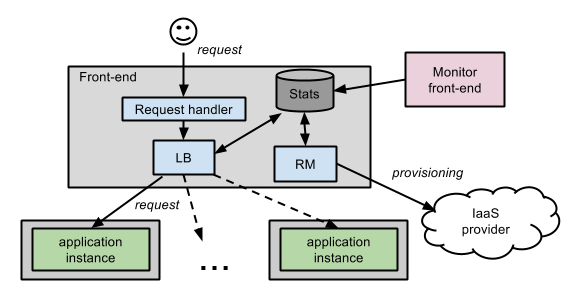
\includegraphics[width=140mm]{architecture_crop.png}
  \caption{High-level system architecture.}
  \label{fig-arch}
\end{figure*}

\subsection{Resource Management Architecture}

The system consists of the following components:

\begin{itemize}
  \item Load balancer (LB): Takes a user request, and passes this off to an application instance based on a scheduling policy (described below).
  \item Resource manager (RM): Periodically polls every application instance to check if it's alive, as well as to retrieve the current load of the system. When it notices the load has become too high or low, it can allocate or deallocate resources based on some provisioning policy (described below).
  \item Monitor front-end: User interface for the usage data collected by the RM.
  \item Application instance: Instances of the image processing application itself. Responds to user HTTP requests.
\end{itemize}

Each application instance runs in its own IaaS machine. The other components run in one centralized component, including permanent storage to store usage statistics for the monitor front-end.

A typical workflow for this system would be the following:

\begin{itemize}
  \item Application delivery: the initial request from a user arrives at the central component, where the load balancer passes it to a suitable instance. The instance responds with a web application where the user may upload an image along with processing parameters.
  \item Job submission: the load balancer shoots the job to an instance (which may be different from the instance that delivered the application).
  \item Job completion: once the instance has completed the job, the user is notified of the result.
\end{itemize}

To keep the system simple, we do not perform any kind of user authentication, and every job is considered to be submitted by a completely new ``user''. We believe this is an acceptable trade-off for this application, which mostly consists of ``one-off'' image processing jobs with a limited running time. However, we are aware that this design limits some of the features we are able to implement.

\subsection{System Policies}

\subsubsection{Load balancing}
The load balancer keeps track of the number of requests active on each instance. This number is referred to as the \emph{load} of an instance. When a new request comes in, the load balancer picks the instance with the least load to pass the request to.

\subsubsection{Provisioning}
In addition to the load per instance, the load balancer also keeps track of the \emph{system load}. The system load is defined as the average of all loads over the instances. We further smooth this metric over a sliding window in order to be less sensitive to short peaks and valleys.

The system load thus calculated is passed to the resource manager, in order to perform provisioning. When the system load becomes higher than a fixed threshold, the provisioner allocates a new instance. Similarly, when the system load becomes lower than a fixed threshold, it deallocates a random existing instance. However, there are set minimum and maximum bounds beyond which the provisioner does not allocate or deallocate.

This is a very simple provisioning policy, which may be optimized further. For example, at the moment we only allocate/deallocate one instance at a time. We chose this policy because it is simple to reason about, and yet works reasonably effectively in our tests. Future versions of the application should explore more sophisticated provisioning policies. The prime example of such a policy would be to use neural networks to learn from previous loads and adjust the number of machines more efficiently.

\subsubsection{Failure handling}
There are two ways in which the system detects failed or unresponsive instances. The first is when the load balancer tries to pass a request to an instance and fails. As a fallback in the case where the instance does not receive requests for a while, we also poll all instances periodically. When the resource manager detects such a failure, it removes the instance from consideration, and tries to allocate a replacement. All requests that were running on the failed instance will return with an error. At this point, the client may resubmit the request.

Assuming image processing tasks are generally rather short running, it will be acceptable to completely restart these kinds of jobs. Future versions of imgCloud may be extended to send failed jobs off to alternative servers for completion in order to provide a better quality of service to the end user.

When the front-end fails, it needs to be manually restarted. On restart, the front-end will ask the IaaS provider for all running instances and rebuild the pool accordingly.


\subsection{Additional System Features}

\subsubsection{User-profiling}
The produced system has support for user profiling by making users ``stick'' to the first application server they use. In order to support this, the application set a cookie with the machine ID on the first request.

As long as the load of the preferred machine is not higher than a configurable threshold, consecutive requests are redirected to this machine. Furthermore the template used to start new instances is configurable based on the instance ID. As the instance ID is strictly incrementing, it is trivial to start all even instances with version A of the code and all odd instances with version B.

\subsubsection{Caching}
In order to provide caching support the application relies on the local storage of each application instance. The results of requests are stored on disk with a filename consisting of a MD5 hash of the unprocessed file as well as the provided processing options. For any request, the application then first checks whether the file has already been processed and if so, it returns the cached result. 

\section{Experimental Results}

\subsection{Experimental setup}
We implemented our design as a prototype application built using Node.js. Node.js \cite{nodejs} is a JavaScript framework using an event-based programming model, which is well suited for handling a large number of concurrent connections. We split the implementation in a front-end server and an application instance, each of which can be run separately. Figure 2 shows a screenshot of the web interface of a running application instance.

\begin{figure}
  \centering
    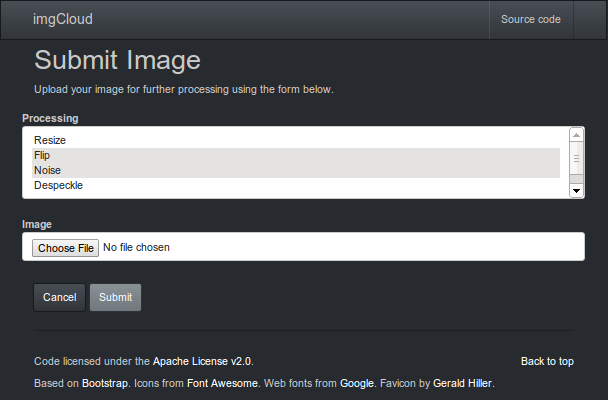
\includegraphics[width=80mm]{imgcloud-screenshot.png}
  \caption{A running application instance.}
\end{figure}

We've released the implementation as an open source project on GitHub \cite{imgcloud} under the MIT license. Instructions on how to run the application can be found in the included README file. The application can be run locally (using one process per instance), or using an IaaS provider (one VM per instance).

To run the experiments, we use DigitalOcean \cite{digital-ocean} as our provider. We've selected this provider because it's relatively cheap and yet provides the features we needed, such as an easy-to-use RESTful API. To bootstrap the experiment, we simply boot one instance and run the front-end. Next, we simulate a workload using Apache JMeter \cite{jmeter}. After the experiment finishes, we retrieve the statistics from the front-end database.


\subsection{Experiment 1 -- Burst workload}
In our first experiment, we created a workload that simulates a steady base workload, with an intermittent burst in order to simulate a sudden, short increase in load. From hereon out we consider our typical user to submit an average of one image per hour.

The base workload consists of 5000 users, submitting a total of 5000 requests per hour. Each request comprises a typical wallpaper-sized image, which needs to be resized and filtered using a motion blur. 

Furthermore, we simulate a, seemingly worst-case, burst load of 30000 users who are active during one hour. This results in a total of 60 concurrent connections. These connections are started 20 seconds after the who are started 20 seconds after the base load has started at a rate of one per second, causing the burst to steadily grow larger. 
The application is set up with one front-end, and 2 initial application instances. We can allocate at most 3 additional instances. In a realistic setting, we reason that we can handle at most around 10 requests per instance before the performance starts to suffer too much. Therefore, we set up the provisioner such that we allocate a new instance when the system loads is at around 8 requests per instance on average. When the system load dips below 2, we deallocate.

In figure \ref{fig-request-distri}, we see the resulting load over time per application instance. Figure \ref{job-makespan} shows the distribution of job makespan throughout the experiment.

\begin{figure}
  \centering
    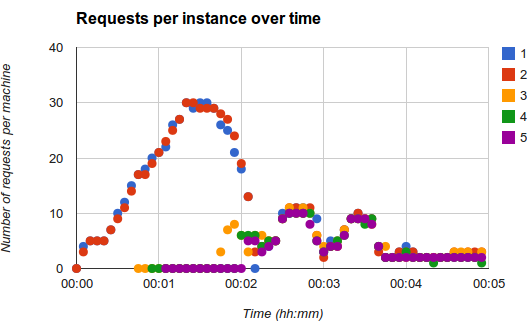
\includegraphics[width=80mm]{requests-per-instance.png}
  \caption{Experiment 1: Request distribution per instance over time.}
  \label{fig-request-distri}
\end{figure}

\begin{figure}
  \centering
    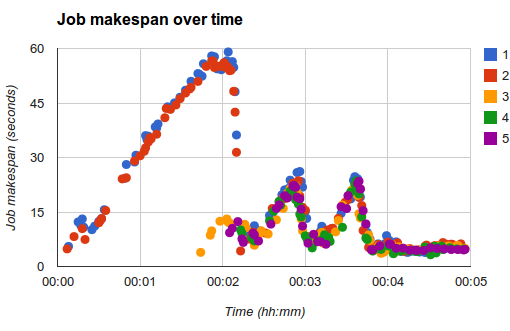
\includegraphics[width=80mm]{job-makespan.png}
  \caption{Experiment 1: Job makespan over time.}
  \label{job-makespan}
\end{figure}

\begin{table}[H]
  \centering
  \begin{tabular}{| l | l | l |}
    \hline
    Charged time & 6 hours \\ \hline
    Charged cost & \euro 0.60 \\ \hline
  \end{tabular}
  \caption{Experiment 1 Metrics}
  \label{exp1-metrics}
\end{table}

In table \ref{exp1-metrics}, we list the experiment metrics for this experiment, according to the charging scheme mentioned in the lab assignment. Although we only used each of the 6 VMs (one front-end, five instances) for a short period of time, each of these VMs is charged as one hour.

\subsubsection{Automation and Elasticity}
When we look at figure \ref{fig-request-distri}, we can see that around 00:00:20 the average instance load exceeds the threshold of 8. This resulted in the allocation of three new machines (3, 4 and 5) in the following 10 second intervals. At around 00:01:45 we observe that machine 3 has finished starting and is accepting new requests. Furthermore, at the 00:04:30 mark the average load dips below the lower threshold of 2, resulting in the deallocation of machine 1. This shows the automatic allocation of new machines, resulting in elastic behavior.


\subsubsection{Performance}

The request from our experiment takes about 5 seconds to complete in an isolated environment. This makespan decreases semi-linearly with the amount of additional requests on the system. For our purposes, we pose that a performance decrease of at most 10x is acceptable without negatively influencing the user experience too much.

In figure \ref{job-makespan}, we see that the maximum makespan increases to about 60 seconds before our provisioner is able to allocate and boot new instances to take over the load. This is an increase of 12x over our base makespan. We note that this unacceptable performance lasts for about 40 seconds before the new instances are able to take over and bring the system load to acceptable levels.


\subsection{Experiment 2 -- Instance failure}
In our second experiment, we focused on reliability of the system in case of failures. We started a typical, steady workload similar to the base workload in experiment 1, and then interacted with the system to test several characteristics.

\subsubsection{Reliability}
With the system running, we simulated a failure by manually killing one of the instances. We observe that, after the next request for this machine fails, the resource manager notices the failure and correctly removes the instance from the resource pool. The resource manager also sends a deallocation request to DigitalOcean to get rid of the VM. In the case of our workload, we only use the minimum amount of instances, which means that the RM allocates a new instance to get us back to our minimum.

Next, we simulated a failure of the front-end server. We observe that all requests fail instantly. After restarting the front-end, all running application instances are discovered and re-added to the pool.


\subsection{Misc. experiments}

There were a few additional features of our application that we tested using specific, focused experiments, which we describe below.

\subsubsection{Monitoring}
During our experiments, we made use of the monitoring dashboard that was running on the front-end server. This monitor provided live insights into the system, including the number of users active on the system, the average load over all instances, the load for each of the instances and the last response time. Example output can be seen in figure \ref{monitoring-dash}.

\begin{figure}
  \centering
    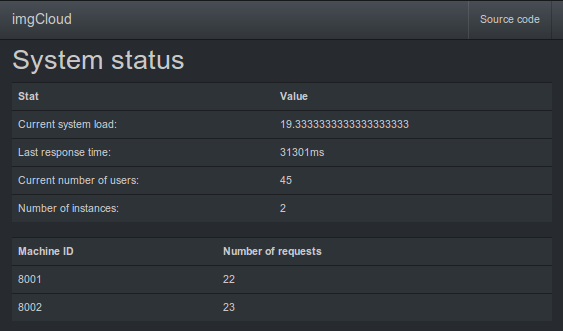
\includegraphics[width=80mm]{imgcloud_dash.png}
  \caption{The monitoring dashboard in action.}
  \label{monitoring-dash}
\end{figure}


\subsubsection{User-profiling}
To test the user-profiling feature, we ran the system and observed that users are consistently assigned to the machine that handled their requests before. In the case of a heavy workload, where we want to prioritize load balancing, the load balancer assigns users to low-load machines, overriding user-profiling, which matches our design. Furthermore, when the machine the user previously used was offline, the preference was ignored and the user was sent to a different machine, to which they stick thereon out.

\subsubsection{Caching}
Finally we have tested the caching behavior. In order to test this we started two instances and submitted a workload consisting of three different images. We observe that the makespan of consecutive identical requests is reduced to tens of milliseconds, limited only by the I/O performance of the host, compared to tens of seconds for regular processing. 

\section{Discussion}
%Summarize the main findings of your work and discuss the tradeoffs inherent in the design of cloud-computing-based applications. Should the WantCloud CTO use IaaS-based clouds? Among others, use extrapolation on the results, as reported in Section 6.b of the report, to discuss the charged time and charged cost reported in section for 100,000/1,000,000/10,000,000 users and for 1 day/1 month/1 year.

\subsection{Results}
We have produced a system that is capable of functioning fully automatic. During this automatic operation imgCloud scales the number of application instances up and down within the limits of admin configurable upper and lower bounds. This behavior is shown to have a beneficial import on the system performance, reducing the job makespan during busy hours. Furthermore it will automatically reduce the number of machines during the less busy times. This results in a significant cost saving when compared to a static allocation of machines. At the same time the application features a generally higher quality of service.

There are of course drawbacks to this approach. During our experiments, we observed an average delay of 60 seconds between machine start and the application being ready to take on work. When taking into account the sliding window used to smooth the system load, this results in an average delay of around 75 seconds between the start of a burst and the arrival of extra capacity. This means that the system is unable to efficiently react to bursts that are this short-lived. Literature suggests that this is a common pattern across various IaaS providers.\cite{mao-vm-startup-time} This leads us to believe that this is a necessary trade-off when it comes to elasticity and is something that can only be addressed by having more capacity on ``stand-by'' to handle the initial load. 

In our case this meant that we had sufficient capacity to handle around 30 seconds of burst load before the performance reaches unacceptable levels. During Experiment 1 this resulted in a 40 second time interval during which the performance was unacceptable according to our definition. After the first additional machine comes online the performance rapidly returns to the regular operational levels, as was shown in figure~\ref{job-makespan}. We feel that a ``bad quality'' interval of less than a minute would be acceptable in practice. 

The system features an architecture that is able to handle failures of the components handling the actual work. When an application instance fails it will not be considered for any follow-up requests. When necessary, a replacement will be allocated. The system does however contain a single point of failure in the form of the central component, housing the Resource Manager. 

Crashes of this software component can be recovered in a limited amount of time through a monitoring demon. Machine failures are more difficult to recover from however. Through the use of a predefined template for this machine it is possible to start a replacement server in a limited amount of time, this does however require an external watchdog. Alternatively, if failures turn out to be likely to happen or too costly to handle, it would be possible to use a cloud load balancer that can rapidly switch between the active central component and a hot-spare backup. Using this approach, failures of this machine could be handled within seconds.

In terms of additional features, the system has support for user profiling. Users are sent to the same machines they previously used as long as the machine is available and not too busy. Furthermore it is trivially possible to specify on a per-instance basis what template should be used on creation, which makes it simple to serve a different application version to a subset of users. 

Furthermore the application features a concise monitoring front-end, which provides insight into various parts of the system such as the last response time, number of instances and more. Besides the web front-end, a script is included to export the logs from the used database, which can easily be imported into third party monitoring tools or spreadsheet applications.

\subsection{Extrapolation}

In our experiments we've been able to demonstrate interesting properties of the system. However, due to constraints, we've only been able to test the system for a limited time, with up to 5 instances, and the workload has only been as large as we could stress the system with this amount of resources. Due to the elasticity, we assume that we can scale the system infinitely given enough resources, with the cost being the only limiting factor.

Assuming again that requests take 5 seconds to complete, and an average user submits 1 requests per hour. When we let each machine process 10 requests at a time, then a single machine can process 7200 requests in an hour (any more than that and we allocate a new instance).

\begin{table}[H]
  \centering
  \begin{tabular}{| l | l | l | l |}
    \hline
    Users & Machines & Charged time (per day) & Charged cost (per day) \\ \hline
    100K & 14 & 336 & \euro 33.60 \\ \hline
    1,000K & 140 & 3360 & \euro 336 \\ \hline
    10,000K & 1400 & 33,600 & \euro 3360 \\ \hline
  \end{tabular}
  \caption{Extrapolation to large amounts of users}
\end{table}

In the extreme case, for 10 million users, this means we would have to spend about \euro 1.2 million on server costs a year, for the average load.

\subsection{Recommendation}
In the context of the kind of image processing application that WantCloud develops, we've seen that a IaaS-based implementation benefits from a number of interesting characteristics. Such an application is capable of scaling up and down depending on the current load. This means that it is possible to support both burst loads and quiet hours while the cost would be comparable to systems that offer lower peak performance. Failures can occur without taking down the entire system. All of this happens completely automatically, and with total insight into the system using the monitor.

There is, of course, a cost involved in outsourcing infrastructure to a IaaS-provider. Nonetheless, we've seen that the costs scale reasonably well even with extreme amounts of users. While the costs of around \euro 1.2 million for just servers at 10M users are significant, this translates to a cost of 12 cents per user per year.

For image processing, we have demonstrated that a IaaS-based implementation is feasible, and in addition we we have presented one possible design that fulfills WantCloud's requirements.

All things considered, we recommend that the WantCloud CTO considers using an IaaS architecture, allowing the company to benefit from the aforementioned advantages offered by such systems.

\section{Conclusion}

We have presented imgCloud, a scalable IaaS-based image manipulation system. The system is shown to be capable of operating in an automatic fashion, during which it can scale its capacity up and down depending on the system load. The system is capable of balancing the incoming load across a range of machines in a fair fashion.

Finally the system is shown to be capable of recovering from faults, offers a wide range of statistics and supports features such as A/B testing. Furthermore we show that the use of a cloud-based solution can provide a decent cost advantage over using a static set of servers.

\section*{Appendix A: Feedback}

Although the assignment did not enforce an IaaS provider, the DAS-4 cluster was recommended in the lab and throughout the course. We decided not to go with the DAS-4 cluster because we had some initial pains with the system, and because prior experience taught us that DigitalOcean is a capable, cheap provider.

Nonetheless, we did have a few minor issues with DigitalOcean, notably when the servers we allocated no longer booted correctly. We solved this by migrating to a different data center region (New York instead of Amsterdam).

\section*{Appendix B: Time sheets}

\begin{table}[H]
  \centering
  \begin{tabular}{| l | l | l |}
    \hline
    Activity & Time \\ \hline
    Total & 110h \\ \hline
    Think & 12h \\ \hline
    Dev & 55h \\ \hline
    Experiment & 10.5h \\ \hline
    Analysis & 3.5h \\ \hline
    Write & 27h \\ \hline
    Wasted & 2h \\ \hline
  \end{tabular}
  \caption{Overall time spent}
\end{table}

The wasted time was spent on diagnosis, contact with support and migration to a different data center zone during the Digital Ocean issues.

\begin{table}[H]
  \centering
  \begin{tabular}{| l | l | l |}
    \hline
    Activity & Time \\ \hline
    Total & 5.5h \\ \hline
    Dev & 4h \\ \hline
    Setup & 1.5h \\ \hline
  \end{tabular}
  \caption{Time spent on Experiment 1}
\end{table}

\begin{table}[H]
  \centering
  \begin{tabular}{| l | l | l |}
    \hline
    Activity & Time \\ \hline
    Total & 3h \\ \hline
    Dev & 2h \\ \hline
    Setup & 1h \\ \hline
  \end{tabular}
  \caption{Time spent on Experiment 2}
\end{table}

\begin{table}[H]
  \centering
  \begin{tabular}{| l | l | l |}
    \hline
    Activity & Time \\ \hline
    Total & 2h \\ \hline
    Dev & 1h \\ \hline
    Setup & 2h \\ \hline
  \end{tabular}
  \caption{Time spent on Experiment 3}
\end{table}

\begin{thebibliography}{6}

\bibitem{image-magick}
ImageMagick. http://www.imagemagick.org

\bibitem{digital-ocean}
Digital Ocean. https://www.digitalocean.com

\bibitem{nodejs}
Node.js. http://nodejs.org

\bibitem{imgcloud}
imgCloud project. https://github.com/mkrause/imgcloud

\bibitem{jmeter}
JMeter. http://jmeter.apache.org

\bibitem{mao-vm-startup-time}
Mao, Ming, and Marty Humphrey. ``A performance study on the vm startup time in the cloud.'' Cloud Computing (CLOUD), 2012 IEEE 5th International Conference on. IEEE, 2012.

\end{thebibliography}

\end{document}
